\documentclass[10pt,twocolumn]{article}

\usepackage[margin=0.72in]{geometry}
\usepackage[T1]{fontenc}
\usepackage[utf8]{inputenc}
\usepackage{lmodern}
\usepackage{microtype}
\usepackage{amsmath,amssymb}
\usepackage{booktabs}
\usepackage{graphicx}
\usepackage{xcolor}
\usepackage{url}
\usepackage[hidelinks]{hyperref}
\usepackage{enumitem}
\usepackage{caption}
\usepackage{balance}

% Avoid conspicuous inter-paragraph stretch when a queued two-column figure
% leaves the current page with unequal natural column heights.
\raggedbottom

\newcommand{\Prob}{\mathbb{P}}
\newcommand{\method}{NLR-QAOA}
\newcommand{\anon}{Anonymous Authors}

\title{When Better QAOA Schedules Depend on the Simulator:\\
Exact and Cross-Backend Rank Reversals on QOBLIB}
\author{\anon\\\small Research draft; author names and affiliations withheld}
\date{}

\begin{document}
\maketitle

\begin{abstract}
Approximate tensor-network simulators extend variational quantum algorithms
beyond the statevector limit, but rankings are often reported at one accuracy
setting. We test ranking stability for depth-15 QAOA schedules on real QOBLIB
Maximum Independent Set benchmarks. On a 186-vertex graph reduced to 55 qubits,
the released Aer MPS setting gives 101 best-known-solution (BKS) hits for a
transferred nonlinear ramp and 41 for the published linear ramp in 15,000 shots
each; tightening only the cutoff reverses the BKS ranking. We then freeze a
five-case exact replication with five MPS settings, three schedules, two qubit
orderings, and Aer and cuTensorNet: 300 dense backend rows, including 240 new
executions. For schedules $i,j$, the event-effect error obeys
$|\widetilde\Delta-\Delta|\leq\mathrm{TV}_i+\mathrm{TV}_j$. All 100 tested
backend/setting/ordering inequalities hold. The certificate
$(\mathrm{TV}_i+\mathrm{TV}_j)/|\Delta|<1$ covers 77 cohorts and all 77 preserve
the exact sign; outside it, only 14 of 23 do (Fisher exact
$p=4.30\times10^{-7}$). Overall sign correctness is 91/100 and cross-backend
sign agreement is 45/50, with all nine sign failures concentrated in the
24-qubit, smallest-margin case. Thus rare-event rankings require
observable-level error budgets rather than a single nominal MPS setting.
\end{abstract}

\section{Introduction}

QAOA alternates problem and mixer Hamiltonians with variational angles chosen
by a classical optimization loop \cite{farhi}. Parameter transfer amortizes
that loop by learning angles on donor instances and deploying them on larger
acceptors \cite{galda,montanez}. This strategy is especially attractive when
the target circuit is too large for exact statevector simulation. In practice,
such targets are often evaluated with approximate tensor networks, whose
runtime and accuracy are controlled by bond dimensions and truncation
thresholds \cite{mpsreview,zerosetup}.

The optimization literature usually asks which QAOA schedule is better. The
simulation literature asks how runtime and aggregate error scale with an
approximation parameter. We ask a question at their intersection:
\emph{does the simulator preserve the ordering of QAOA schedules on the
observable used to declare a winner?} This is not guaranteed. The probability
of an optimum may live in a small tail of the output distribution; a small
state approximation error can therefore cause a large relative error in that
rare-event probability without visibly changing average energy or feasibility.

We study this issue on the Quantum Optimization Benchmarking Library (QOBLIB),
a curated, submission-oriented framework designed for reproducible comparison
of quantum and classical optimization methods \cite{qoblib}. We reproduce the
released depth-15 Aer/MPS pipeline for the \texttt{es60fst02} Maximum
Independent Set (MIS) instance, including graph reduction, Hamiltonian
construction, sample unfolding, and a validity-only filter. We compare its
published linear-ramp schedule with a low-dimensional nonlinear ramp selected
on other full ES60FST instances.

Our contributions are:
\begin{enumerate}[leftmargin=*,nosep]
  \item a train-validation-test protocol over four complete QOBLIB graphs,
  ending in a 55-qubit, depth-15 blind benchmark with no repair or target
  retuning;
  \item an equal-budget comparison of evolutionary and random schedule search,
  showing that the random-search champion, not the evolutionary operator,
  transfers best;
  \item 15 paired MPS jobs at the published simulator setting, with bootstrap
  intervals and an exact paired randomization test;
  \item a bond/threshold sensitivity audit that identifies a truncation-induced
  BKS rank reversal while near-optimal and feasible-mass rankings remain stable;
  and
  \item dense exact adjudication on five real QOBLIB kernels (3--24 qubits),
  followed by a frozen 300-row Aer/cuTensorNet replication; and
  \item an observable-level TVD certificate that preserves the exact ranking in
  all 77 certified cohorts and isolates all nine observed failures outside the
  certified region.
\end{enumerate}

We do not claim quantum advantage, an exact simulation of the 55-qubit state,
or universal superiority of the nonlinear ramp. The main claim is about
benchmark validity: schedule rankings based on rare optimum hits can depend on
the truncation setting, backend implementation, and qubit ordering even when
all circuits are exactly equivalent before truncation.

\section{Background and related work}

\paragraph{Parameter transfer and schedule reduction.}
QAOA parameters concentrate across related random graphs, motivating donor
selection, representation learning, and direct parameter transfer
\cite{galda,montanez}. Weighted-problem studies show that rescaling phase
angles can restore transfer when coefficient distributions change
\cite{sureshbabu}. Linear-ramp QAOA compresses $2p$ angles to two increments
and has been studied at larger depths \cite{lrqaoa}. Recent constrained-QAOA
work promotes penalty schedules and piecewise ramps to variational parameters
\cite{penaltyschedule}. Our nonlinear ramp is intentionally modest; it is a
vehicle for testing ranking stability, not the central theoretical novelty.

\paragraph{Evolutionary variational optimization.}
Evolutionary methods are natural for nonconvex, noisy quantum objectives
\cite{de}. We use a fixed-population genetic search and compare it with uniform
random search under exactly the same number of candidate evaluations. The
negative result---matched random search finds the stronger transferring
schedule---prevents attributing the observed gain to evolution itself.

\paragraph{Approximate tensor-network simulation.}
MPS simulation compresses a many-qubit state by truncating Schmidt spectra;
accuracy depends on circuit ordering, entanglement growth, the maximum bond
dimension, and discarded-weight policy \cite{mpsreview}. Recent work studies
tensor-network surrogates for variational circuits and the compute-accuracy
frontier of approximate simulators \cite{tnsurrogate,zerosetup}. Exact
tensor-network sampling methods have also reached structured QAOA circuits
beyond conventional statevector sizes \cite{pilotwave}. These studies motivate
careful convergence analysis, but they do not establish that optimization
algorithm rankings are invariant under the approximation controls used in a
submitted benchmark.

\section{Benchmark protocol}

\subsection{Instances and frozen split}

Table~\ref{tab:instances} lists the four full QOBLIB ES60FST MIS instances.
The split was frozen before evaluation of any new schedule on
\texttt{es60fst02}. Best-known values are exact Gurobi optima in the QOBLIB
submission records.

\begin{table}[t]
\centering
\caption{Full QOBLIB instances and quantum kernels at maximum retained degree
four. V/E are original vertices/edges; $n_q/m_q$ are reduced vertices/edges.}
\label{tab:instances}
\small
\begin{tabular}{lrrrrl}
\toprule
Instance & V & E & $n_q$ & $m_q$ & Role / BKS \\
\midrule
es60fst01 & 123 & 159 & 15 & 21 & train / 60 \\
es60fst03 & 113 & 142 & 12 & 16 & train / 55 \\
es60fst04 & 162 & 238 & 45 & 69 & validation / 78 \\
es60fst02 & 186 & 280 & 55 & 91 & blind test / 88 \\
\bottomrule
\end{tabular}
\end{table}

We use the released reduction implementation: sequential exact degree-0/1
rules, exact degree-2 folding, recorded pruning of vertices above degree four,
and a final exact cleanup. Pruning is heuristic; all decisions are recorded so
samples can be unfolded. On \texttt{es60fst02}, 37 vertices are forced selected,
38 forced excluded, 28 folds occur in four batches, and five vertices are
heuristically pruned. The published workflow also uses this 55-qubit kernel and
reaches BKS 88 under Aer MPS \cite{qoblibmps}.

\subsection{Hamiltonian, circuit, and schedules}

For graph $G=(V,E)$, the MIS QUBO is
\begin{equation}
C(x)=-\sum_{i\in V}x_i+\lambda\sum_{(i,j)\in E}x_ix_j,
\qquad \lambda=1.5.
\end{equation}
After $x_i=(1-Z_i)/2$, QAOA alternates the Ising cost operator and
$H_M=\sum_i X_i$. Both methods use depth $p=15$, maximum-quadratic-coefficient
Hamiltonian scaling from the released code, an initial $|+\rangle^{\otimes n}$
state, and identical measurement conventions. The untranspiled test circuit
contains 1,365 RZZ, 825 RZ, 825 RX, 55 Hadamard, and 55 measurement operations.

The published linear ramp is
\begin{equation}
\beta_k=0.7\frac{p-k+1}{p},\qquad
\gamma_k=0.4\frac{k}{p}.
\end{equation}
The candidate family generalizes the ramp with two powers:
\begin{align}
\beta_k &= \Delta_\beta\left(\frac{p-k+1}{p}\right)^{a_\beta},\\
\gamma_k &= \Delta_\gamma\left(\frac{k}{p}\right)^{a_\gamma}.
\end{align}
The four-dimensional genome lies in
$\Delta_\beta\in[0.15,1.20]$, $\Delta_\gamma\in[0.05,1.00]$, and
$a_\beta,a_\gamma\in[0.30,2.50]$. The frozen random-search champion is
$(0.64247,0.75939,1.77679,0.99172)$; the evolutionary champion is
$(0.51750,0.77197,1.07734,1.75435)$.

\subsection{Search, selection, and metrics}

Three independent search replicates use 20 candidates for six generations,
or 120 candidate evaluations per method. Each candidate receives 256 shots on
each training instance. Random search receives exactly 120 independently drawn
candidates. A finite-shot robust score combines Wilson lower bounds on BKS,
BKS-1, and feasible probabilities with feasible quality mass; its mean and
worst-instance values are combined 3:1. One validation pass on
\texttt{es60fst04} selects one champion per search method. Test outcomes are
never used for schedule selection.

For every reduced sample, the released decoder reverses folds and forced
decisions. We retain the full sample only if it is already an independent set.
There is no constraint repair, greedy fill, local search, or archived-solution
fallback. We report
\begin{itemize}[leftmargin=*,nosep]
  \item BKS hit probability $\Prob(|S|\geq88)$;
  \item near-BKS probability $\Prob(|S|\geq87)$;
  \item feasible probability; and
  \item quality mass $\mathbb{E}[\mathbf{1}_{\rm feasible}\min(|S|/88,1)]$.
\end{itemize}

The confirmatory run uses 15 paired simulator seeds and 1,000 shots per method
and seed. Paired mean differences receive a 20,000-draw bootstrap interval and
an exact two-sided sign-flip test over all $2^{15}$ paired sign assignments.

\subsection{Independent backend and classical controls}

We export the frozen native circuits to NVIDIA cuTensorNet 26.6
\cite{cuquantum}. Direct contraction reproduces Qiskit statevectors for both
schedules on both 12- and 15-qubit kernels with fidelity one to displayed
precision. The 55-qubit exact sampler fails during network preparation, so all
completed large-circuit results are explicitly approximate MPS results. We use
a Fiedler-vector qubit ordering, exact-equivalent before truncation, that lowers
edge bandwidth from 47 to 10 and maximum linear cut from 42 to 9. We test bond
128 with discarded-weight cutoffs $10^{-3}$ and $10^{-4}$ using 5,000 shots per
schedule. Samples are inverse-permuted before the unchanged decoder is applied.

Classical controls operate on the original full graph and on the released
55-variable kernel. An exact binary MILP is solved with SciPy/HiGHS at zero MIP
gap. A randomized minimum-residual-degree heuristic repeatedly selects a
minimum-degree vertex with random tie breaking, deletes it and its neighbors,
and uses no archived solution. Both heuristic variants receive 15,000 starts.

\subsection{Simulator settings and audit}

The primary setting exactly follows the submission: Qiskit Aer MPS, maximum
bond dimension 64, truncation threshold $10^{-3}$, and native RZ/RZZ/RX
circuits with no hardware-basis transpilation. This detail matters because a
gate decomposition changes when MPS truncation is applied. A first transpiled
pass was preserved as a protocol audit and excluded from the main result.

We then hold circuits and shots fixed while testing thresholds $10^{-3}$,
$3\times10^{-4}$, and $10^{-4}$ at bond 64, plus bonds 64 and 96 at thresholds
$10^{-3}$ and $10^{-4}$. Audit points use 10,000 shots per principal method;
the primary $10^{-3}$/64 point aggregates 15,000 shots.

To calibrate the direction and magnitude of approximation error, we also run
complete statevectors on the real 12- and 15-qubit training kernels. For both
principal schedules we compare exact probabilities with MPS states at bond
dimensions 16, 32, 64, and 128 and thresholds from $10^{-3}$ to $10^{-6}$.
We report state fidelity, total-variation distance, Jensen-Shannon divergence,
and signed errors in BKS, near-BKS, feasibility, and quality mass. These are
probability-exact comparisons with no measurement noise.

\subsection{Exact external adjudication and cross-backend ladder}

After the 55-qubit study, we froze a separate exact cross-case experiment on
five real QOBLIB instances: \texttt{karate}, \texttt{chesapeake},
\texttt{football}, \texttt{ibm32}, and \texttt{aves-sparrow-social}. Their
frozen reductions contain 3, 7, 7, 18, and 24 qubits. We evaluate the published
LR, prior evolutionary, and prior matched-random depth-15 schedules under
sorted and spectral qubit orderings. Dense statevectors enumerate every
outcome; the QOBLIB unfolding and feasibility rules are compiled into bit
literals and accumulated without shots or repair.

The independent ladder fixes five points before execution: bond/cutoff
$(64,10^{-3})$, $(128,10^{-4})$, $(128,10^{-12})$,
$(1024,10^{-4})$, and $(1024,10^{-5})$. The six native circuits are exported as
hashed QPY files to cuTensorNet 26.6. Both backends return dense approximate
states, which are normalized and compared with the six exact states by fidelity,
total variation, and application metrics. The design contains exactly
$5\ \text{cases}\times5\ \text{settings}\times3\ \text{schedules}\times
2\ \text{orderings}\times2\ \text{backends}=300$ dense rows. The completed
60-row 24-qubit cohort was reused only after SHA-256 validation; the other 240
rows were executed after the cross-case protocol was frozen. The primary
estimand is the sign of matched-random-minus-LR BKS probability; incomplete
cohorts are not interpreted.

For BKS event $A$, exact distributions $p_i,p_j$, and approximate distributions
$q_i,q_j$, we pre-specify the observable-rank certificate
\begin{equation}
|[q_i(A)-q_j(A)]-[p_i(A)-p_j(A)]|
\leq \mathrm{TV}(q_i,p_i)+\mathrm{TV}(q_j,p_j).
\label{eq:tvd-cert}
\end{equation}
The exact sign is certified whenever $|p_i(A)-p_j(A)|$ exceeds the right-hand
side. Its derivation and complete cohort table are provided in the Supplement.

\section{Results}

\subsection{Search method is not the source of the gain}

On the 45-qubit validation kernel, the evolutionary champion raises feasible
probability from 0.561 to 0.930 but lowers BKS probability from 0.040 to 0.017.
The matched-random champion attains 0.941 feasibility, 0.051 BKS, and 0.475
near-BKS. This result was fixed before the corrected blind pass. It shows that
the nonlinear family contains transferable schedules, but the evolutionary
operator does not outperform a matched random search at this budget.

\subsection{Published MPS setting}

Table~\ref{tab:blind} and Fig.~\ref{fig:blind} summarize 45 method-jobs on the
blind instance. All methods find BKS 88 in every aggregate. The random-search
nonlinear ramp improves all four reported rates relative to the published
linear ramp. It produces 101 BKS hits versus 41, and its BKS advantage is
positive in 13 seeds with two ties and no losses. The estimated shot count for
a 95\% chance of at least one BKS sample,
$\lceil\log(0.05)/\log(1-p_{\rm BKS})\rceil$, falls from 1,095 to 444.

\begin{table}[t]
\centering
\caption{Blind \texttt{es60fst02} results at bond 64 and threshold $10^{-3}$;
15,000 shots per method.}
\label{tab:blind}
\small
\begin{tabular}{lrrrr}
\toprule
Method & BKS & BKS-1 & Feasible & Quality \\
\midrule
Published LR & .00273 & .11213 & .50127 & .48962 \\
Evolutionary & .00207 & .06813 & .89987 & .87202 \\
Matched random & \textbf{.00673} & \textbf{.15700} & \textbf{.90180} & \textbf{.87865} \\
\bottomrule
\end{tabular}
\end{table}

\begin{figure*}[t]
\centering
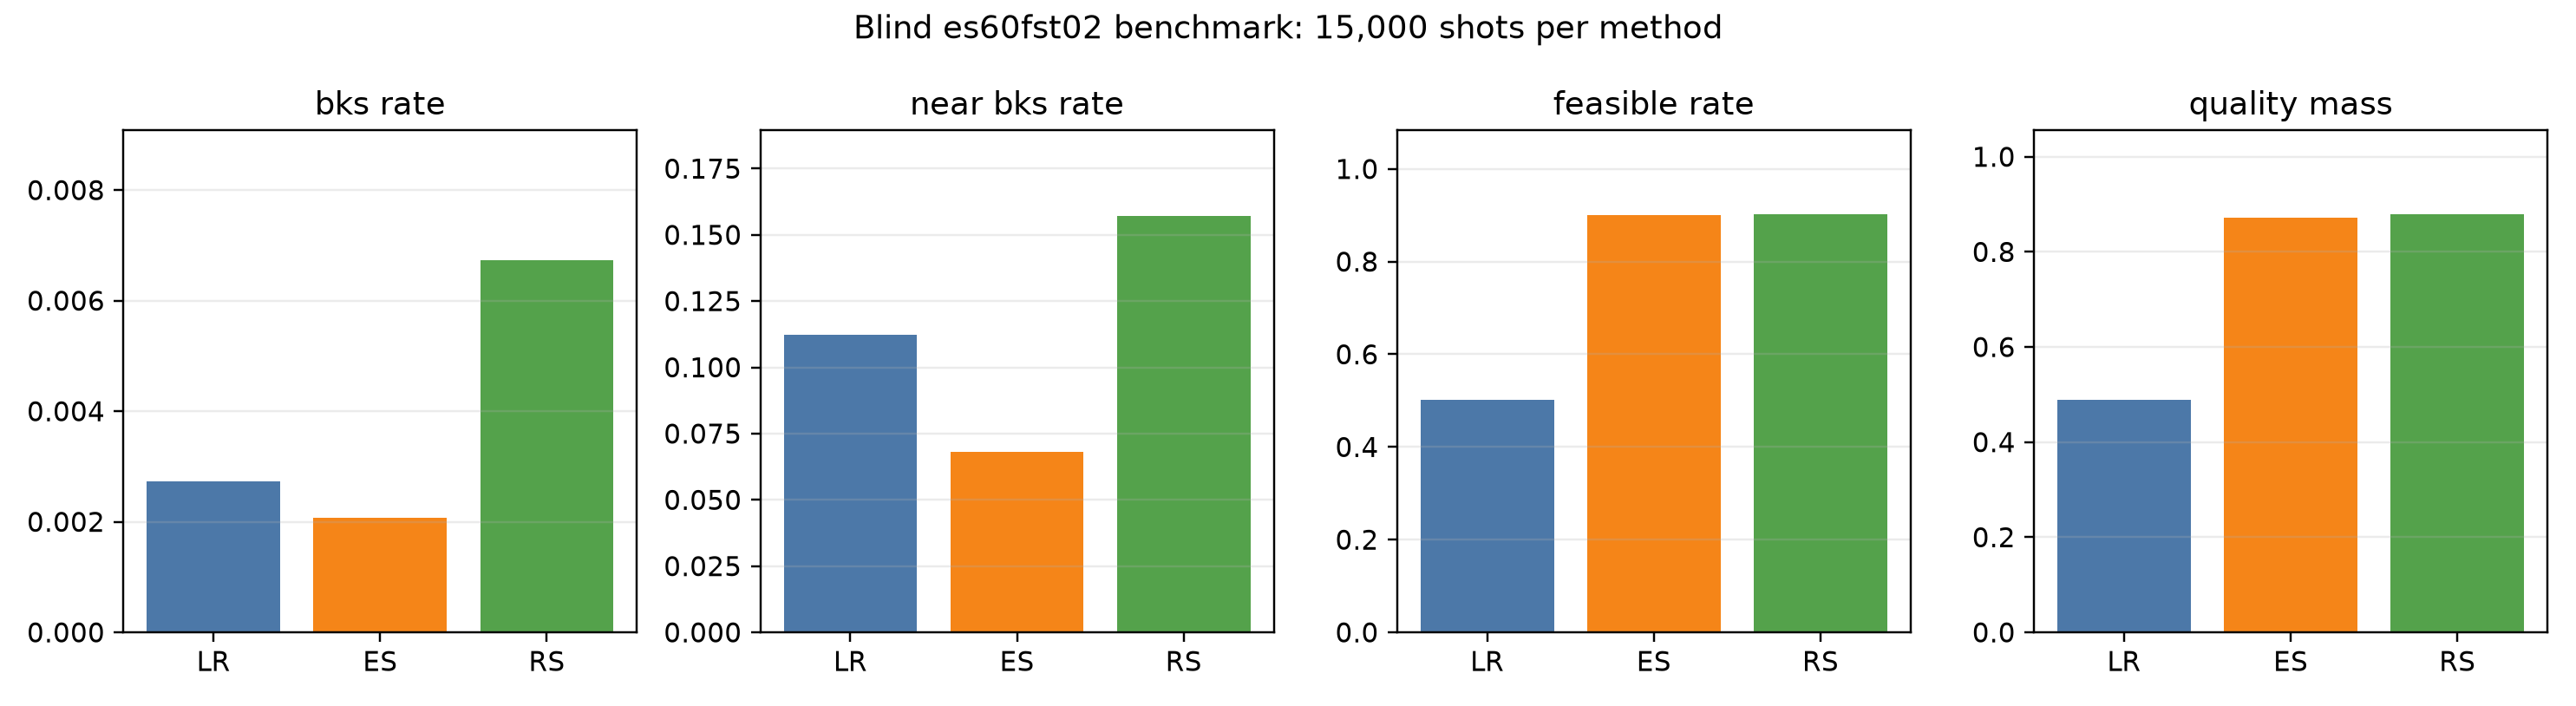
\includegraphics[width=\textwidth]{../results/figures/blind_method_comparison.png}
\caption{Blind metrics at the released Aer/MPS setting. LR is the published
linear ramp; ES and RS are the frozen evolutionary- and random-search nonlinear
ramps. Bars aggregate 15 paired jobs and 15,000 shots per method.}
\label{fig:blind}
\end{figure*}

For matched random minus published LR, the paired BKS difference is $0.00400$
(bootstrap 95\% CI $[0.00247,0.00553]$, sign-flip $p=0.000244$). Corresponding
differences are $0.04487$ for near-BKS, $0.40053$ for feasibility, and $0.38904$
for quality mass; all three have sign-flip $p=6.10\times10^{-5}$. The
evolutionary champion improves feasibility and quality mass but not BKS or
near-BKS, reinforcing the negative optimizer result.

\subsection{Truncation-induced rank reversal}

Figure~\ref{fig:sensitivity} shows the central finding. At bond 64 and threshold
$10^{-3}$, the nonlinear ramp has the larger BKS rate. At $3\times10^{-4}$ it
still leads, 0.0161 to 0.0116. At $10^{-4}$ the order reverses: published LR
reaches 0.0153 and the nonlinear ramp 0.0109. The shot-noise standard error of a
rate near 0.01 with 10,000 shots is approximately 0.001, smaller than the
observed 0.0044 gap.

The same threshold tightening does not reverse the broader metrics. At
$10^{-4}$/64, nonlinear versus LR is 0.1621 versus 0.1546 for near-BKS and
0.7351 versus 0.4809 for feasibility. At $10^{-4}$/96 it is 0.1808 versus
0.1710 near-BKS and 0.7121 versus 0.4799 feasible. The optimum-hit tail is thus
more ranking-sensitive than near-optimal or feasible mass.

\begin{figure*}[t]
\centering
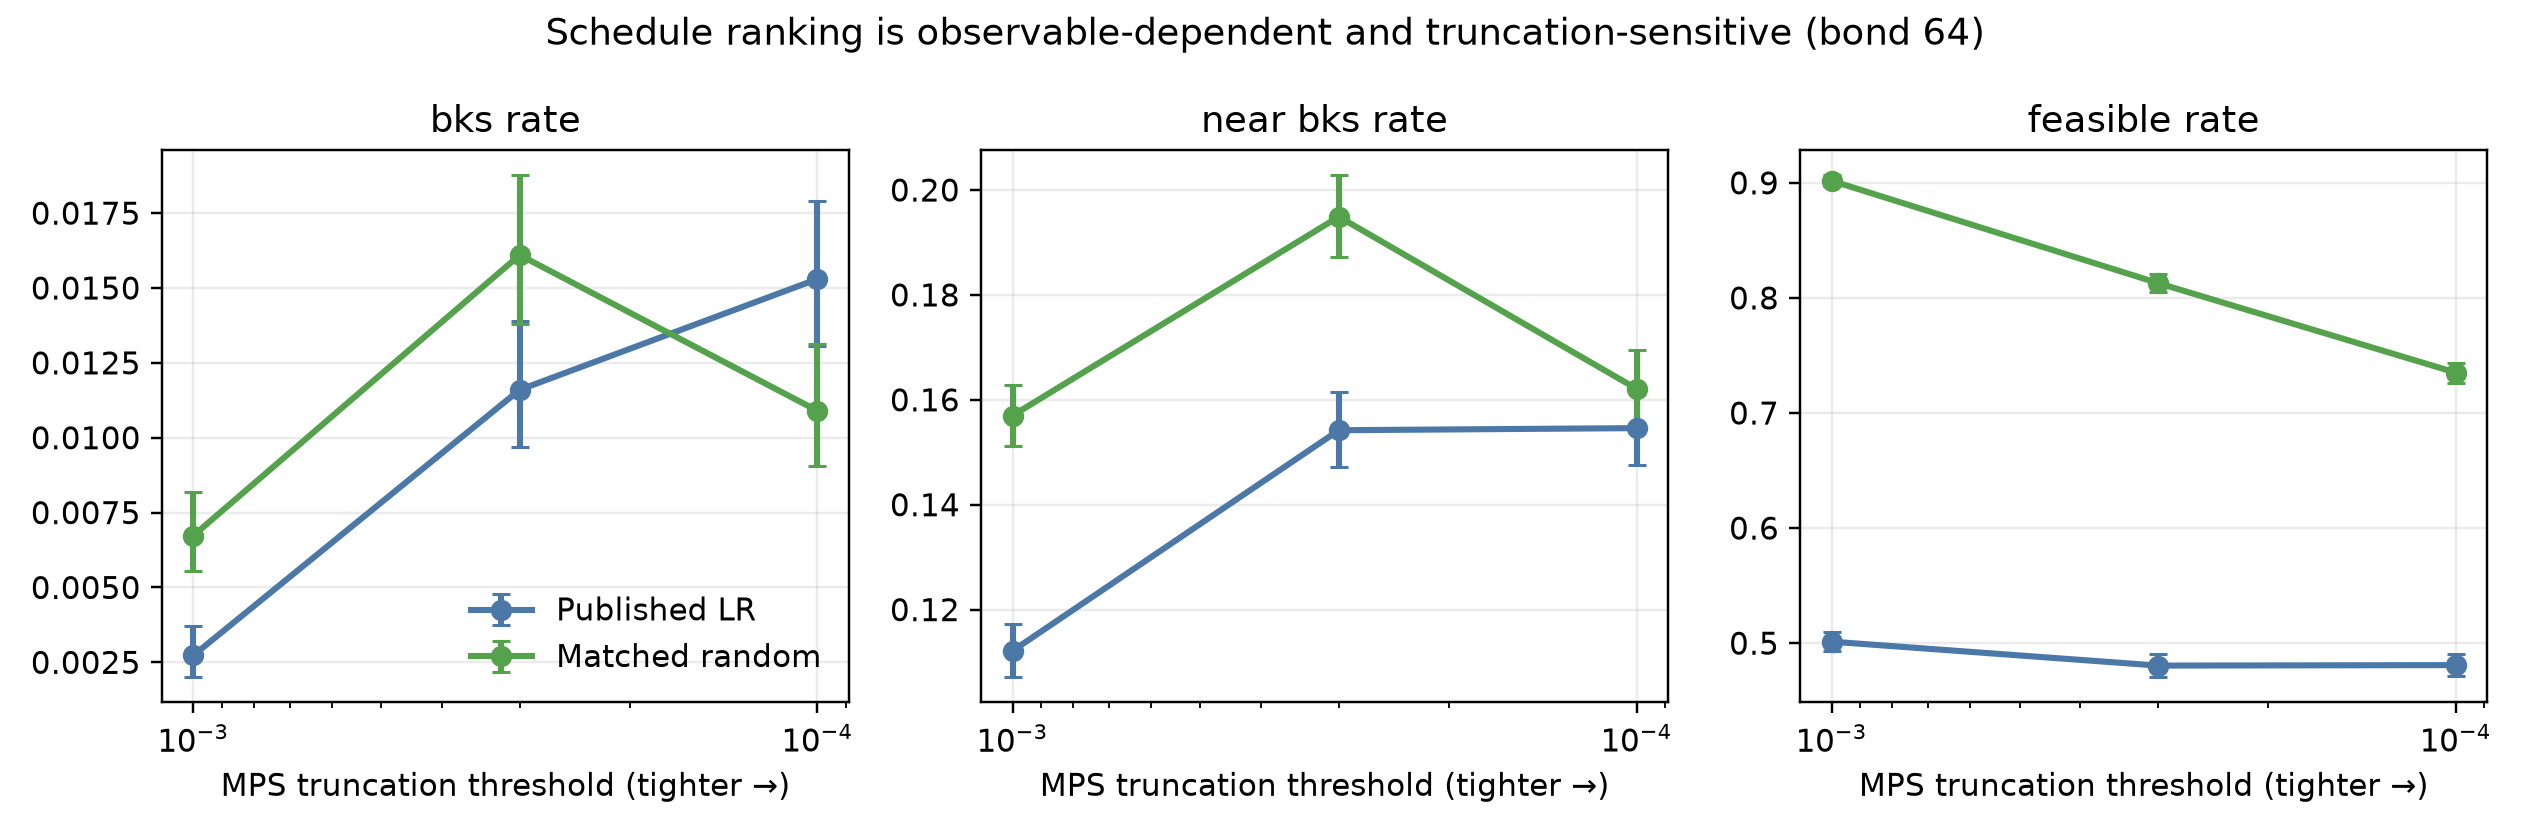
\includegraphics[width=\textwidth]{../results/figures/mps_threshold_sensitivity.png}
\caption{Observable-dependent convergence at fixed bond dimension 64. Tightening
the threshold reverses the BKS ranking between $3\times10^{-4}$ and $10^{-4}$,
while near-BKS and feasible rankings remain unchanged. The $10^{-3}$ point uses
15,000 shots; the other points use 10,000 shots per method.}
\label{fig:sensitivity}
\end{figure*}

Increasing the bond cap alone does not explain the effect. At threshold
$10^{-3}$ and bond 96, nonlinear still leads BKS 0.0070 to 0.0019, near-BKS
0.1661 to 0.1188, and feasibility 0.8925 to 0.5055. At threshold $10^{-4}$ and
bond 96, the BKS comparison is 0.0134 versus 0.0152, again favoring LR, while
near-BKS and feasibility continue to favor nonlinear. The threshold is the
dominant control in the tested range.

Runtime makes this audit consequential rather than cosmetic. At bond 96,
tightening the threshold from $10^{-3}$ to $10^{-4}$ increases the two-circuit
batch from about 38 seconds to about 347 seconds on the local CPU. An attempted
bond-128, $10^{-6}$ three-method batch exceeded 20 minutes and was terminated
without producing a result. Single-setting reports therefore create a real
temptation to use a cheap but unconverged point.

\subsection{Exact-state calibration isolates threshold bias}

The small-kernel calibration supplies ground truth for the same schedules and
reduction family. On \texttt{es60fst01}, exact BKS probabilities are 0.68610
for LR and 0.92898 for the nonlinear ramp. At threshold $10^{-3}$, MPS shifts
them by $+0.01577$ and $+0.03417$, respectively. On \texttt{es60fst03}, exact
BKS probabilities are 0.73583 and 0.95530; corresponding MPS biases are
$+0.00744$ and $+0.01849$. Thus, the released threshold overstates BKS
probability for both schedules but more strongly for the nonlinear ramp.

Figure~\ref{fig:calibration} shows convergence. At $10^{-3}$, total-variation
distance is 0.0518/0.0509 for LR and 0.0742/0.0702 for nonlinear on the two
kernels. At $10^{-6}$ all four state fidelities exceed 0.99983, total variation
is below 0.00266, and absolute BKS error is below 0.00023. For shared
thresholds, results are numerically identical at bonds 32, 64, and 128. Bond 16
differs only for the nonlinear \texttt{es60fst01} circuit at $10^{-4}$, where
total variation changes by less than 0.0005. Thus, once the cap reaches 32, the
discarded-weight threshold controls the error. The nonmonotonic signed BKS error for LR also shows
why convergence of a rare observable cannot be inferred solely from a
monotonically improving global state metric.

\begin{figure*}[t]
\centering
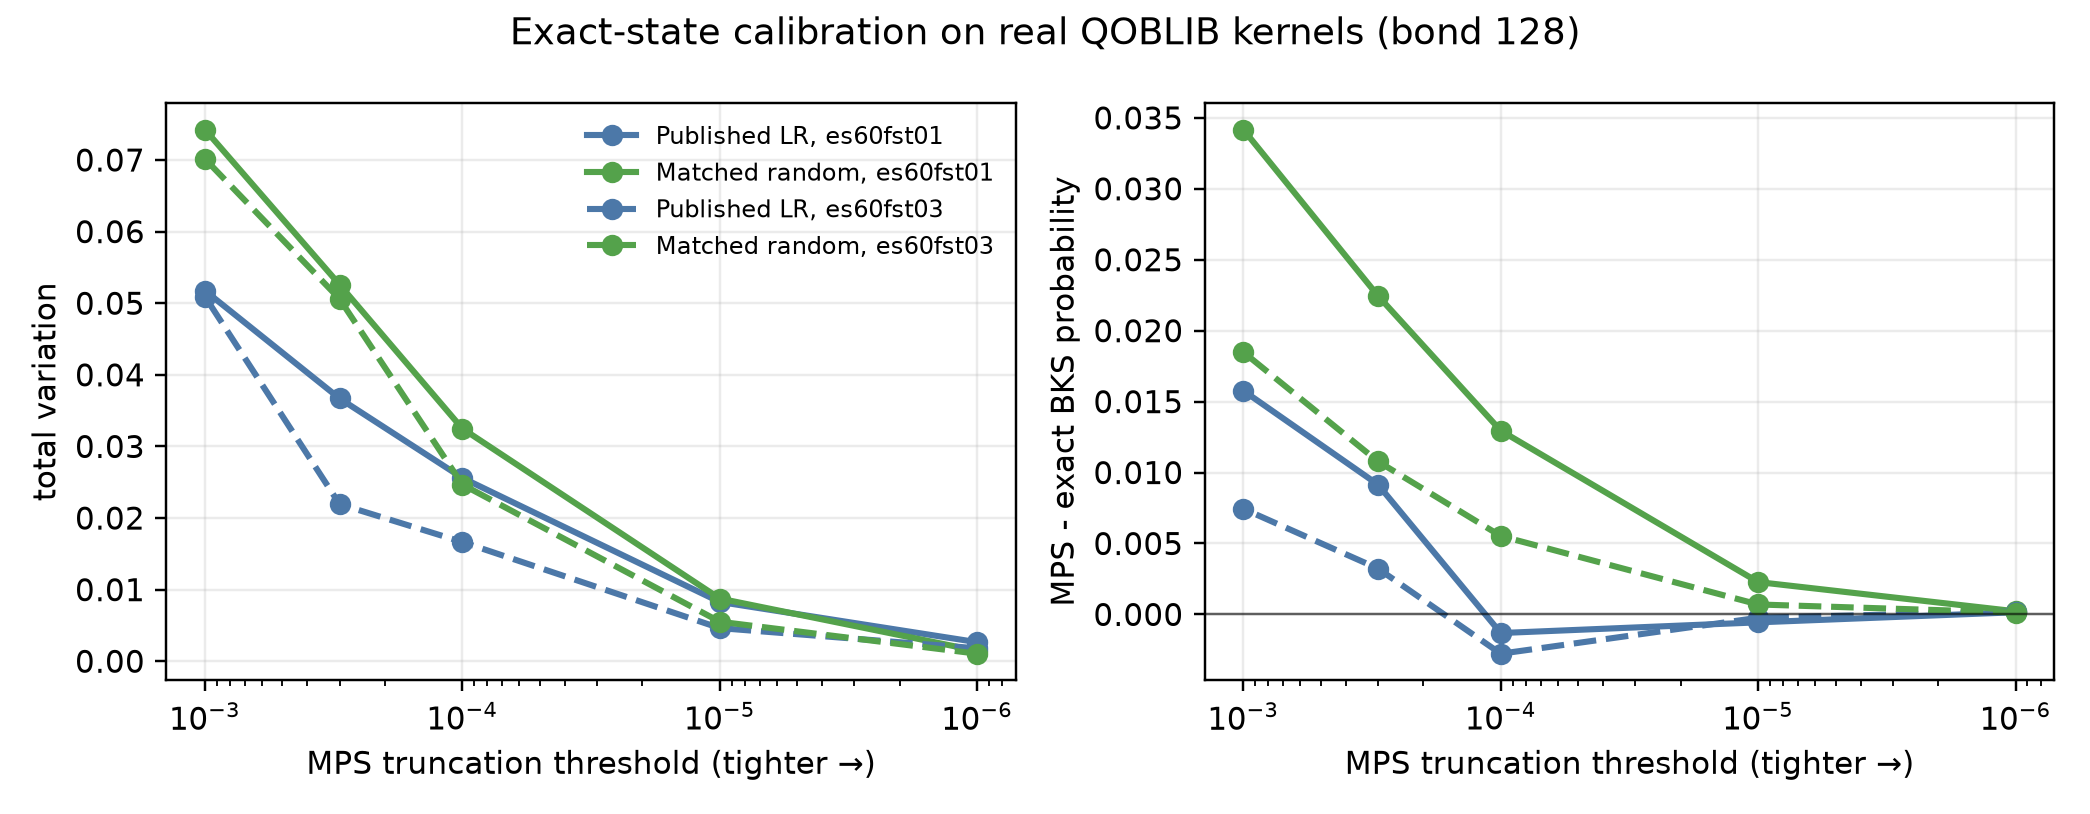
\includegraphics[width=0.92\textwidth]{../results/figures/exact_mps_calibration.png}
\caption{Exact-state MPS calibration on the 15-qubit \texttt{es60fst01} and
12-qubit \texttt{es60fst03} kernels at bond 128. Left: total-variation distance
from the exact output distribution. Right: signed error in BKS probability.
Tightening the truncation threshold drives both errors toward zero, but the
rare-event bias is schedule-dependent and need not be monotone.}
\label{fig:calibration}
\end{figure*}

\subsection{Cross-case replication and rank certificate}

The five exact matched-random-minus-LR BKS effects are $+0.086412$ for
\texttt{karate}, $-0.134214$ for \texttt{chesapeake}, $+0.019269$ for
\texttt{football}, $-0.246123$ for \texttt{ibm32}, and $-0.012139$ for
\texttt{aves-sparrow-social}. The design therefore spans both effect signs,
3--24 qubits, and a 20-fold range of nonzero effect magnitudes.

Figure~\ref{fig:crosscase} summarizes all 100 backend/setting/ordering cohorts.
Equation~\ref{eq:tvd-cert} holds in every cohort; the largest numerical excess
of observed error over its bound is $6.6\times10^{-16}$, consistent with
floating-point accumulation. Overall, 91/100 approximate matched effects have
the exact sign and Aer/cuTensorNet agree in 45/50 matched cohorts. The exact
margin exceeds the TVD error budget in 77/100 cohorts. Every one of these 77
certified cohorts is sign-correct (Clopper--Pearson 95\% lower bound 0.953),
whereas 14/23 uncertified cohorts are correct. This contrast is descriptive but
large (two-sided Fisher exact $p=4.30\times10^{-7}$); the guarantee itself comes
from Eq.~\ref{eq:tvd-cert}, not from the test.

The per-case pattern supports an effect-margin explanation rather than a qubit
count rule. \texttt{karate} and \texttt{chesapeake} are universally certified
from the released point; \texttt{football} first becomes universal at the
confirm point and \texttt{ibm32} at bond 1024/cutoff $10^{-4}$. All 80 cohorts
on these four cases preserve the exact sign, including three conservative false
negatives of the certificate. The smallest-margin 24-qubit case accounts for
all nine sign failures and all five cross-backend sign disagreements. Its
tightest setting is sign-correct in all four backend/order combinations but is
still not universally TVD-certified, illustrating that a sufficient
certificate need not be necessary.

\begin{figure*}[t]
\centering
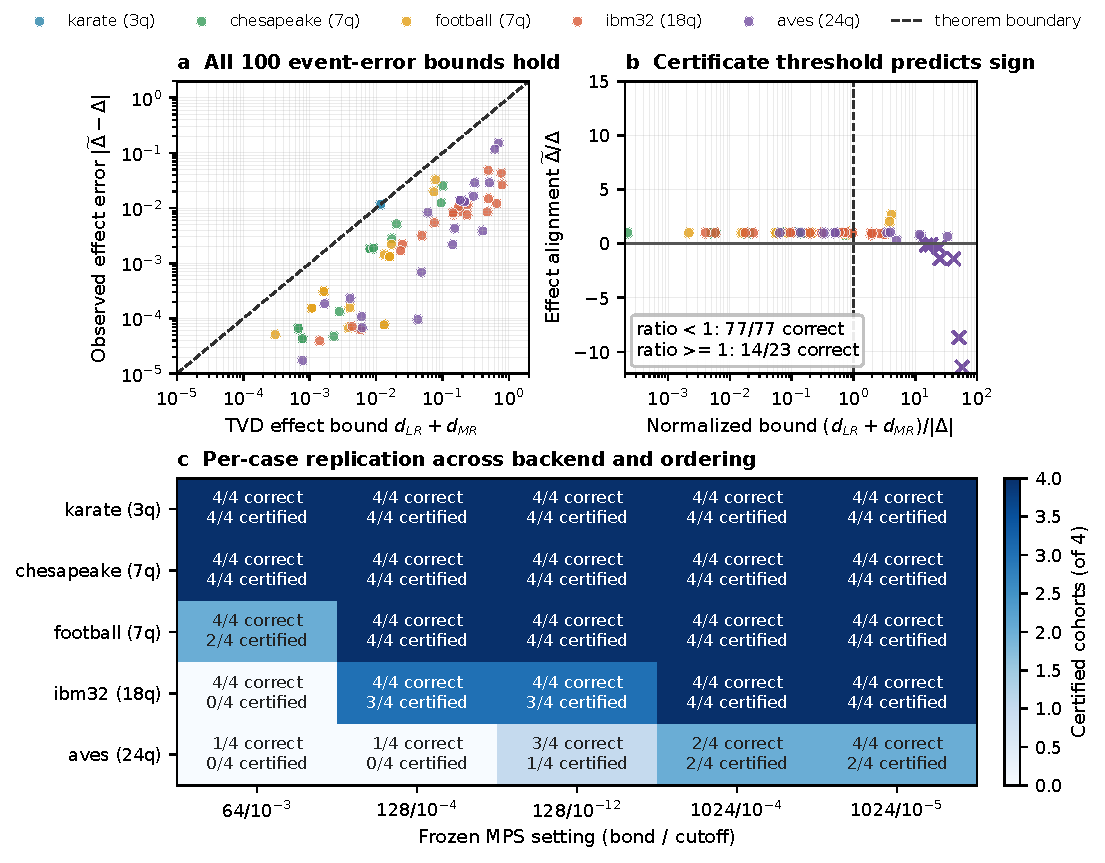
\includegraphics[width=0.98\textwidth]{../results/figures/cross_case_replication.pdf}
\caption{Frozen five-case exact replication. (a) Observed matched-effect error
never exceeds the sum of schedule TVDs. (b) The normalized TVD budget provides
a deterministic sign certificate below one; crosses mark wrong-sign cohorts.
(c) Correct and certified cohorts among the four backend/order combinations at
each case and MPS setting.}
\label{fig:crosscase}
\end{figure*}

\subsection{Exact 24-qubit cross-backend adjudication}

The exact 24-qubit BKS probabilities are 0.323277 for LR, 0.311138 for the
matched-random schedule, and 0.425256 for the evolutionary schedule. They are
invariant to the two exact-equivalent qubit orderings. Thus the exact
matched-random-minus-LR effect is $-0.012139$: the small positive advantages
seen at several approximate settings have the wrong sign.

Figure~\ref{fig:independent} gives all ten matched-effect cohorts. At the
released point Aer reports $+0.138479$ and $+0.105273$ for sorted and spectral
ordering. cuTensorNet instead reports $-0.008287$ and $+0.016849$, so even the
direction of the error is backend- and ordering-dependent. The nominal confirm
point remains sign-wrong for both Aer orderings and for spectral cuTensorNet.
At bond 128 with cutoff $10^{-12}$ Aer has the correct sign in both orderings,
whereas cuTensorNet does so only in sorted order.

The sharpest cross-backend result occurs at bond 1024 and cutoff $10^{-4}$:
cuTensorNet has the correct sign in both orderings, minimum state fidelity
0.997210, and maximum BKS error 0.000150, while Aer has the wrong sign in both.
Only cutoff $10^{-5}$ gives the correct sign for every tested backend and
ordering. At that point cuTensorNet's minimum fidelity is 0.999982 and maximum
BKS error is 0.000229; Aer's corresponding minimum fidelity is 0.990609. A
named bond/cutoff pair therefore does not define a portable accuracy level
across MPS implementations.

Across 20 backend/setting/ordering cohorts, 11 realized signs are correct but
only five satisfy the stricter TVD margin certificate; all five are correct.
The complete certificate audit is given in the Supplement.

\begin{figure*}[t]
\centering
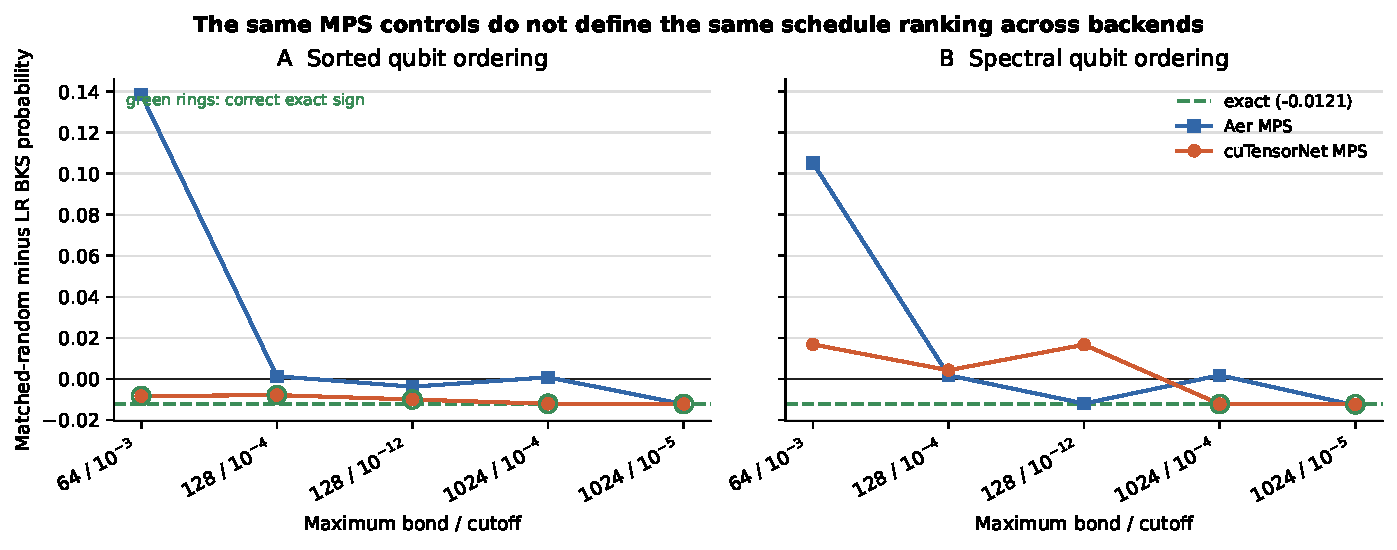
\includegraphics[width=0.88\textwidth]{../results/figures/independent_ladder.pdf}
\caption{Exact-calibrated matched-random-minus-LR BKS effects on the 24-qubit
\texttt{aves-sparrow-social} kernel. The dashed line is the dense exact effect;
green rings mark cuTensorNet points with its correct sign. Aer and cuTensorNet
can disagree in sign at the same nominal bond/cutoff, and qubit ordering changes
the approximate ranking despite exact equivalence.}
\label{fig:independent}
\end{figure*}

\subsection{55-qubit independent backend and classical controls}

At spectral ordering and bond 128, independent cuTensorNet MPS yields 15 versus
6 BKS hits for nonlinear versus LR at cutoff $10^{-3}$ in 5,000 shots per
method: rates 0.0030 and 0.0012 (two-sided Fisher exact $p=0.078$). Tightening
to $10^{-4}$ removes that directional advantage: counts are 11 versus 12,
rates 0.0022 and 0.0024 ($p=1.0$). Near-BKS changes from 0.0820 versus 0.0424
to 0.0782 versus 0.0764, while feasible probability remains higher for
nonlinear, 0.6232 versus 0.4840 and 0.6352 versus 0.4838. Thus the independent
backend does not reproduce a significant LR advantage at the tighter point,
but it does reproduce loss of the nonlinear BKS advantage while the feasible
ranking remains stable.

The classical comparison rules out a solver-advantage interpretation. HiGHS
proves BKS 88 with zero gap in 0.036 seconds. On the full 186-vertex graph,
randomized minimum-degree greedy produces 1,133 BKS solutions in 15,000 starts
(0.07553) in 19.95 seconds. On the same QOBLIB kernel used by QAOA, it produces
6,063 (0.4042) in 2.21 seconds. These BKS rates are 11.2 and 60.0 times the best
QAOA rate. One third of the measured three-method QAOA batch wall time is about
183 seconds, so the corresponding classical heuristic runs are also about 9.2
and 82.9 times faster. The contribution is therefore diagnostic methodology,
not quantum or heuristic optimization advantage.

\section{Discussion}

\subsection{Why a rank reversal is plausible}

MPS compression repeatedly removes small Schmidt components. BKS probability
is a rare-event functional of the final distribution rather than a smooth
global norm. A schedule can therefore appear superior because the simulator
retains or discards a small set of amplitudes differently. Tightening the
threshold changes BKS probability by factors of several for both schedules,
yet feasibility changes far less for LR and remains much higher for the
nonlinear ramp. This pattern is consistent with rare optimum strings being more
sensitive than broad feasible regions. The exact-state calibration supports
this mechanism directly: global distribution error falls smoothly as the
threshold tightens, while signed BKS error is schedule-specific and crosses
zero for LR.

The 55-qubit experiment does not identify which schedule is closer to its exact
state. Convergence there would require tighter settings, an independent exact
sampler, or quantum-hardware evidence. The five-case exact replication resolves
the mechanism across a broader range: large-margin cases remain sign-stable,
while failures concentrate where the accumulated event-error budget exceeds
the exact schedule margin. The correct general conclusion remains that a BKS
ranking is not established by a single approximate setting.

The independent backend strengthens this statement. On the exact-calibrated
24-qubit case, changing implementation or qubit ordering changes the sign at
fixed nominal MPS controls. Across all cases, cross-backend sign agreement is
45/50 rather than automatic. The cutoff needed for agreement is therefore an
empirical property of the backend--circuit--observable triple, not a portable
fidelity specification. Qubit ordering and backend version must be reported
alongside the usual MPS truncation controls.

\subsection{Implications for optimization benchmarks}

We recommend that approximate-simulator submissions report:
\begin{enumerate}[leftmargin=*,nosep]
  \item native circuit, qubit ordering, bond cap, discarded-weight threshold,
  and whether a basis transpilation was applied;
  \item at least three accuracy points bracketing the reported setting;
  \item ranking stability for every headline observable, not only average
  energy or a simulator fidelity proxy;
  \item an exact-state or independent-backend anchor whenever the target size
  permits one;
  \item an observable-level error budget, such as the TVD rank certificate,
  when a winner is declared by a probability difference;
  \item raw counts, shot budgets, and confidence intervals for rare-event
  metrics; and
  \item a distinction between conclusions stable across settings and those
  conditional on one released benchmark configuration.
\end{enumerate}

These requirements complement QOBLIB's standardized reporting objective
\cite{qoblib}. They also matter for transfer learning: an approximate simulator
can influence not only final evaluation but validation-time model selection.
Our champions were deliberately frozen after a documented code audit, and the
first transpiled run remains archived rather than silently deleted.

\subsection{Limitations}

The transfer study uses one four-instance graph family and one MIS reduction
policy. The
high-degree pruning step is heuristic, although all reported samples are valid
on the original graph and BKS values refer to the full instances. Only two
principal schedules receive the full 55-qubit threshold sweep. For that circuit
we do not compute state fidelity, discarded-weight accumulation, or exact
probabilities. Direct cuTensorNet contraction matches the small exact controls
but its 55-qubit exact sampler returns an internal preparation error; the
independent large-circuit results remain approximate. The dense replication
adds five exact instances but covers five selected MPS points, three frozen
schedules, and two software backends on one GPU. Its 100 cohorts are not
independent statistical samples of a population: settings and orderings share
circuits, so the Fisher test is descriptive and the TVD theorem is the primary
support. Both simulators are noiseless and neither constitutes hardware
evidence. Finally, the
10,000-shot sensitivity points are single simulator jobs, so their binomial
precision is high but job-to-job implementation effects are not separately
estimated.

\section{Reproducibility}

The experiment records Python, Qiskit, Aer, cuTensorNet, NumPy, operating-system metadata,
the cloned baseline commit, and a SHA-256 digest of the frozen protocol.
Training, validation, blind testing, the discarded transpilation audit, every
fidelity point, independent-backend job, and classical run are separate JSON
artifacts. Checkpoints are written after long jobs. The test suite verifies
the published ramp formula, split disjointness, the 186-to-55 reduction,
disabled repair, balanced blind artifacts, exact calibration, classical
feasibility, cuTensorNet axis conventions and unit-fidelity controls, the two
5,000-shot points, completeness of the 300-row replication, and NumPy-safe
artifact serialization. Analysis scripts regenerate CSV tables and all five
figures; export manifests hash every new QPY circuit, exact state, reused
artifact, runner, and frozen protocol.

\section{Conclusion}

On a real 186-vertex QOBLIB instance executed as a 55-qubit, depth-15 QAOA
circuit, a transferred nonlinear ramp appears to improve optimum-hit
probability by 2.46 times at the released MPS setting, but the ranking reverses
when the truncation threshold is tightened. A frozen five-case, 300-row dense
replication then shows 91/100 correct signs and only 45/50 cross-backend sign
agreements. The observable-level TVD certificate is decisive: all 77 certified
cohorts preserve the exact ranking, while every failure lies outside the
certificate. Strong classical controls dominate in both success rate and
runtime. The broader lesson is methodological, not a claim of quantum
advantage. When approximate simulation stands between a variational algorithm
and a benchmark claim, convergence of the \emph{ranking observable} is part of
the algorithm evaluation, not an optional simulator appendix.

\balance
\begin{thebibliography}{99}
\scriptsize
\setlength{\itemsep}{-1.5pt}
\setlength{\parsep}{0pt}

\bibitem{farhi}
E. Farhi, J. Goldstone, and S. Gutmann,
``A Quantum Approximate Optimization Algorithm,'' arXiv:1411.4028 (2014).

\bibitem{galda}
A. Galda et al., ``Similarity-Based Parameter Transferability in the Quantum
Approximate Optimization Algorithm,'' arXiv:2307.05420 (2023).

\bibitem{montanez}
J. A. Montanez-Barrera, D. Willsch, and K. Michielsen,
``Transfer learning of optimal QAOA parameters in combinatorial optimization,''
Quantum Information Processing 24, 129 (2025).

\bibitem{sureshbabu}
S. H. Sureshbabu et al., ``Parameter Setting in Quantum Approximate
Optimization of Weighted Problems,'' Quantum 8, 1231 (2024).

\bibitem{lrqaoa}
J. A. Montanez-Barrera et al., ``Toward a linear-ramp QAOA protocol: evidence
of a scaling advantage in solving some combinatorial optimization problems,''
npj Quantum Information 11 (2025).

\bibitem{penaltyschedule}
F. Ferrari, M. Vandelli, and D. Dragoni, ``Feasibility-driven QAOA with penalty
scheduling,'' arXiv:2606.25117 (2026).

\bibitem{de}
R. Storn and K. Price, ``Differential Evolution---A Simple and Efficient
Heuristic for Global Optimization over Continuous Spaces,'' Journal of Global
Optimization 11, 341--359 (1997).

\bibitem{qoblib}
T. Koch et al., ``The Quantum Optimization Benchmarking Library,'' Nature
Computational Science 6, 653--671 (2026).

\bibitem{qoblibmps}
J. A. Montanez-Barrera, ``QAOA Aer/MPS solution for QOBLIB es60fst02,'' QOBLIB
submission 20260611 (2026), \url{https://github.com/ZIB-AOPT/QOBLIB}.

\bibitem{mpsreview}
U. Schollwock, ``The density-matrix renormalization group in the age of matrix
product states,'' Annals of Physics 326, 96--192 (2011).

\bibitem{tnsurrogate}
R. Watanabe, D. Sels, and J. Tindall, ``Tensor network surrogate models for
variational quantum computation,'' arXiv:2604.20180 (2026).

\bibitem{zerosetup}
A. R. Mazumder, M. Z. Mullath, and H. Tepanyan, ``Benchmarking Zero-Setup
Quantum Circuit Simulators,'' arXiv:2607.09882 (2026).

\bibitem{pilotwave}
G. Kalachev et al., ``Pilot-Wave Simulator: Exact Classical Sampling from Ideal
and Noisy Quantum Circuits up to Hundreds of Qubits,'' Quantum 10, 2173 (2026).

\bibitem{cuquantum}
H. Bayraktar et al., ``cuQuantum SDK: A High-Performance Library for
Accelerating Quantum Science,'' 2023 IEEE International Conference on Quantum
Computing and Engineering (QCE), 1050--1061 (2023).

\end{thebibliography}

\end{document}
